\documentclass[12pt,a4paper,spanish]{article} 

\usepackage{graphicx} %option specific for pdfLatex compilation
\usepackage{makeidx}
\usepackage{lscape}

\usepackage[spanish]{babel}
\usepackage[utf8]{inputenc} 
\usepackage{indentfirst}

\usepackage[margin=1in]{geometry}


\begin{document}
\begin{titlepage}
\begin{center}

% Upper part of the page. The '~' is needed because \\
% only works if a paragraph has started.

\textsc{\LARGE \textbf{Universidad de Buenos Aires}}\\%[1cm]
\vfill
\textsc{\LARGE \textbf{Técnicas de Programación Concurrente I }}\\%[0.5cm]
\vfill
\textsc{\LARGE \textbf{(75.59)}}\\%[0.5cm]
\vfill
% Title
%\HRule \\[0.4cm]
\vfill
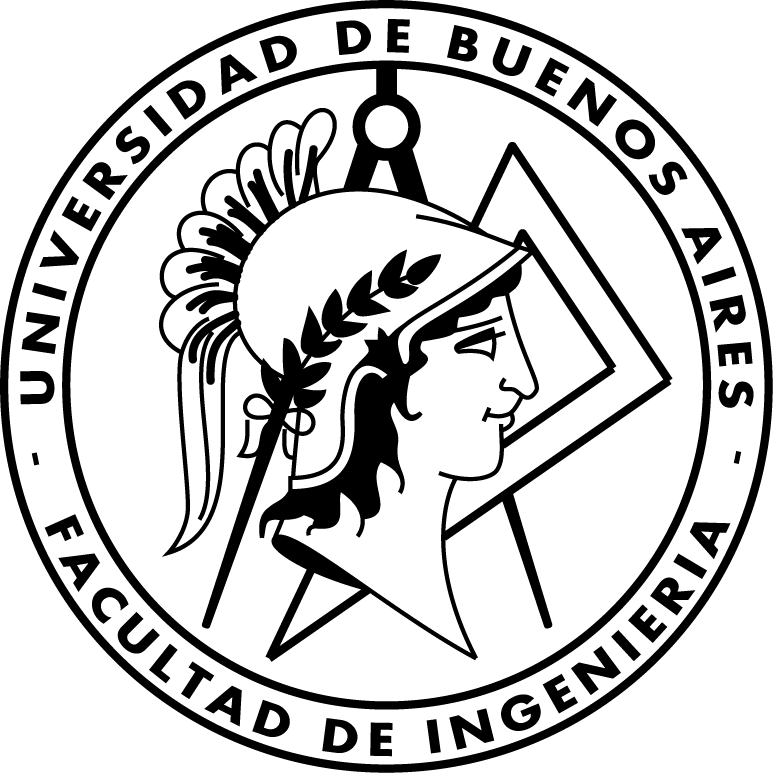
\includegraphics[scale=1.25]{./logo.png}~\\[2cm]
%\HRule \\[1.5cm]
{ \huge \bfseries Trabajo Práctico Nº 1}\\%[0.25cm]
\vfill
%{ \huge \bfseries Grupo 8}\\%[0.25cm]
%\vfill
{\Large
\begin{tabular}{|c|c|c|}
\hline
Nombre y apellido & Padrón & Mail \\
\hline
Florencia Bosch & 91867 & florb\_128@hotmail.com \\
\hline
Javier Choque & 92079 & javierchoque21@gmail.com \\
\hline
Pablo Musumeci & 92165 & pablomusumeci@yahoo.com.ar\\
\hline
\end{tabular}
}
\vfill

% Bottom of the page
{\large \today}

\end{center}
\end{titlepage}

\newpage
\tableofcontents
\newpage
\section{Diseño}

\section{Hipótesis}

\begin{itemize}
	\item Consideramos que cuando un auto es enviado a la salida por el Jefe de Estación,
	el mismo sale del sistema de manera instantánea, sin tener que hacer una cola
	para salir de la estación.
\end{itemize}

\subsection{Casos de uso}

\begin{itemize}
	\item Inicar simulación: El actor que dispara este caso de uso es el usuario
	que desea iniciar la simulación. Para iniciar el programa se debe ejecutar el
	proceso \texttt{procesoPrincipal}, el cual se encarga de
	lanzar a los otros procesos involucrados en el funcionamiento de la simulación.

	Es necesario que la ejecución del proceso principal se realize con los parámetros
	que indican la cantidad de empleados (por medio de la expresión \texttt{-e} o \texttt{--empleados})
	y la cantidad de surtidores (\texttt{-s} o \texttt{--surtidores})que que tendrá la
	estación de servicio.

	Ejemplo:

	\texttt{./procesoPrincipal -e 5 -s 7}
\end{itemize}

\section{Procesos}

	\subsection{Generador de Autos}
		
		Este proceso es el encargado de crear los autos que llegan a la estación. Para
		dicho propósito, genera cada una cierta cantidad de tiempo aleatorio, un nuevo
		auto (compuesto por un ID y una cantidad de dinero que va a gastar en al estación).

		El Generador de Autos interactua con el Jefe de Estación, y dicha interacción se puede
		asemejar al problema \textbf{Producer - Consumer}, debido a que, el Generador produce
		los autos que el Jefe de Estación va a recibir. 

		Al analizar este problema, debemos tener en cuenta que el \textbf{producer} no debería
		agregar información al buffer que comparte con el consumer, si el mismo se encuentra lleno.
		En esta situación nosotros optamos por enviar a dormir al proceso generador, por un tiempo
		aleatorio, y volver a intentar escribir en el buffer cuando se despierte.

	\subsection{Jefe de Estación}
		Este proceso se encarga de recibir los autos nuevos que van llegando a la estación. 
		En este caso, el Jefe de Estación es el \textbf{consumer} de información, y debe
		cerciorarse de no intentar extraer información del buffer si el mismo esta vacío.

		Una vez que logró extraer un automóvil del buffer exitosamente, debe asignarle 
		un empleado al auto recibido, en caso de que exista algun empleado disponible 
		en ese mismo instante, caso contrario,deberá redirigir el mismo hacia la salida.

	\subsection{Empleado}

	\subsection{Empleado}


\end{document}
